\chapter{Estudio Previo}\label{cap:05EstudioPrevio}

En esta sección se muestra un estudio comprensivo del estandar OHDSI utilizado: qué es, su ......

\section{Introducción}

El trabajo fin de grado se basa en OHDSI

\section{¿Qué es OHDSI?}

OHDSI, pronunciado en inglés ''Odyseey'', son las siglas de Observational Health Data Science and Informatics. OHDSI es una organización colaborativa de ciencia abierta cuyo propósito, de forma muy resumida, es mejorar la investigación cientifico-sanitaria a través de la ciencia de datos y la informática clínica. No obstante, no es solo una organización, sino una comunidad global abierta a todo el que esté interesado y alineado con su misión, visión y objetivos. 

La comunidad se asigna por tanto la misión de ''mejorar la salud empoderando a una comunidad para generar de manera colaborativa evidencia que promueva mejores decisiones de salud y una mejor atención'', y comparte la visión de ''un mundo en el que la investigación observacional produzca una comprensión integral de la salud y la enfermedad'' \cite{OHDSIwebsite}\cite{OHDSIbook}. 

Por otra parte, en \textit{El Libro de OHDSI} la organización se define así misma como ''una comunidad de ciencia abierta que tiene como objetivo mejorar la salud empoderando a la comunidad para generar de manera colaborativa evidencia que promueva mejores decisiones de salud y mejor atención'' \cite{OHDSIbook}. La web oficial presenta otra definición algo diferente, se presenta como ''una colaboración de ciencia abierta, interdisciplinaria y de múltiples partes interesadas para resaltar el valor de los datos de salud a través de análisis a gran escala'' \cite{OHDSIwebsite}.

\begin{figure}[H]
    \centering
    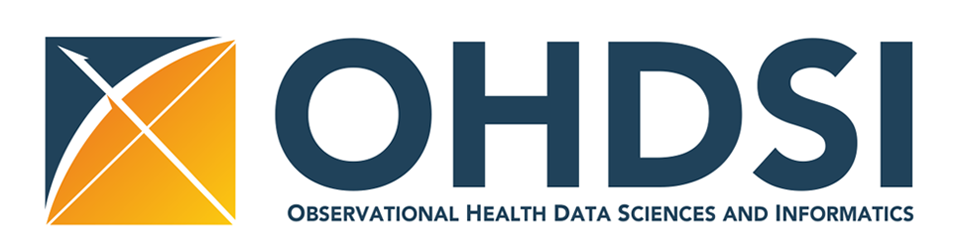
\includegraphics[width=0.90\textwidth]{figures/OHDSIbanner.png}
    \caption{Banner de OHDSI. Extraído de web oficial \cite{OHDSIwebsite}}
    \label{fig:enter-label}
\end{figure}

De esta forma se pueden inferir tres características fundamentales de la organización: (i) ser una comunidad o red colaborativa, (ii) ser de ciencia abierta y (iii) tener la finalidad de promover la extracción de evidencia a partir de datos clínicos.

\begin{enumerate}[label=\roman*.]
    \item La organización es una comunidad, siempre abierta a la incorporación de nuevos colaboradores, lo que muestran con el eslogan \textit{''Join the Journey''}, en español, ''únete a la aventura''. En los capítulos 2.1 y 2.2 del \textit{Libro de OHDSI} se presenta una guía de cómo unirse a la comunidad y participar de sus múltiples eventos. Pero además, OHDSI no es solo una comunidad localizada en un único punto, sino una red colaborativa con múltiples nodos en diferentes países y continentes que comparten el mismo objetivo. Por tanto, los eventos que realiza OHDSI generalmente son de carácter internacional como grupos de trabajo, llamadas comunitarias semanales o los symposium anuales, entre otros.

    \item Además, todos estos eventos y el trabajo que elabora la red son abiertos, puesto que OHDSI es una organización de ''ciencia abierta''. Todos los eventos, publicaciones, herramientas y documentación están disponibles públicamente y de forma gratuita en internet, para que pueda unirse quien quiera (en el caso de los eventos) o consultarse y usarse en cualquier momento (en caso de las herramientas e información). La organización se mantiene económicamente a través del Centro de Coordinación Central, situado en el Centro Médico Irving de la Universidad de Columbia, que es quien asume los costes asociados a la infraestructura central y la coordinación comunitaria por medio del apoyo de los miembros de la comunidad y del patrocinio \cite{OHDSIwebsite}.

    \item Por último, destacar la finalidad de OHDSI de promover la importancia de, no solo recopilar y almacenar la información clínica sino también extraer información o evidencia de ella, que es lo que se denomina comunmente ''el uso secundario de los datos''. Para ello, promueve también la importancia de establecer una metodología estándar para la realización de dichos estudios e investigaciones científicas, persiguiendo \textcolor{red}{los principios FAIR }y favoreciendo la reciclabilidad y reproducidad de los estudios. Gracias a la ciencia abierta, OHDSI promueve a sus colaboradores llevar a cabos sus estudios mediante las herramientas de tratamiento de datos que ofrece y el modelo común de OMOP, fundamentalmente.
    
    
\end{enumerate}

\subsection{Historia}

Es común encontrar en internet los términos OHDSI y OMOP (\textit{Observational Medical Outcomes Partnership}), utilizados de forma casi indistintiva. Si bien es verdad que OMOP se suele asociar mayoritariamente al CDM (\textit{Common Data Model}) también OHDSI mantiene gran relación con este modelo común de datos. Entonces, ¿cuál es la relación entre estas dos entidades? 

La iniciativa de OHDSI se origina en 2014, posterior al proyecto OMOP, que finalizó en 2013, pues la relación que guardan estas dos entidades es parental, OHDSI es la sucesora de OMOP.

OMOP nació en 2008 como una asociación público-privada presidida por la Administración de Alimentos y Medicamentos de EE. UU. con el objetivo de establecer buenas prácticas en estudios observacionales retrospectivos. El proyecto además fue administrado por la Fundación de los Institutos Nacionales de Salud y financiado por un consorcio de compañías farmacéuticas en colaboración con otros investigadores académicos y socios de datos de salud \cite{stang2010advancing}. El propósito inicial de OMOP era impulsar la ciencia de la vigilancia activa de la seguridad de los productos médicos mediante el análisis de datos observacionales de atención médica \cite{stang2010advancing}. Sin embargo, durante su desarrollo, se enfrentó a los desafíos técnicos de llevar a cabo investigaciones en bases de datos observacionales muy heterogéneas entre sí.

El resultado fue el desarrollo de un Modelo Común de Datos (CDM) como un mecanismo para estandarizar la estructura, el contenido y la semántica de los datos observacionales y hacer posible escribir código de análisis estadístico que fuera reutilizable para estudios en distintas fuentes de datos \cite{overhage2012validation}. Los experimentos de OMOP demostraron la viabilidad de establecer un CDM que además reuniese diferentes vocabularios estandarizados, reuniendo en un mismo estándar diversos tipos de datos de diferentes entornos de atención y representados por diferentes vocabularios de origen. Esta característica facilitó la colaboración y aumentó el interés entre diferentes instituciones lo que promovió o un enfoque de ciencia abierta \cite{OHDSIbook}. OMOP puso todo su trabajo a disposición del público, incluidos diseños de estudio, estándares de datos, código de análisis y hallazgos empíricos, para mejorar la transparencia y fomentar la confianza en su investigación. 

Al término del proyecto, el Modelo Común de Datos (CDM) de OMOP había evolucionado hasta respaldar un abanico  amplísimo de aplicaciones analíticas, incluida la efectividad comparativa de intervenciones médicas y políticas de todo el sistema de salud, no solo de la industria farmacéutica, por tanto, el equipo de investigación acordó que el fin de dicho proyecto debería ser el origen de uno nuevo. a partir de esta idea nació OHDSI \cite{OHDSIbook}.

\subsection{Actualidad}

Por tanto, lo que nació en 2014 como la continuación del proyecto OMOP ha evolucionado hasta convertirse en una extensa red colaborativa global.  En la actualidad, cuenta con la participación de más de tres mil colaboradores distribuidos en 80 países.

\begin{figure}[H]
    \centering
    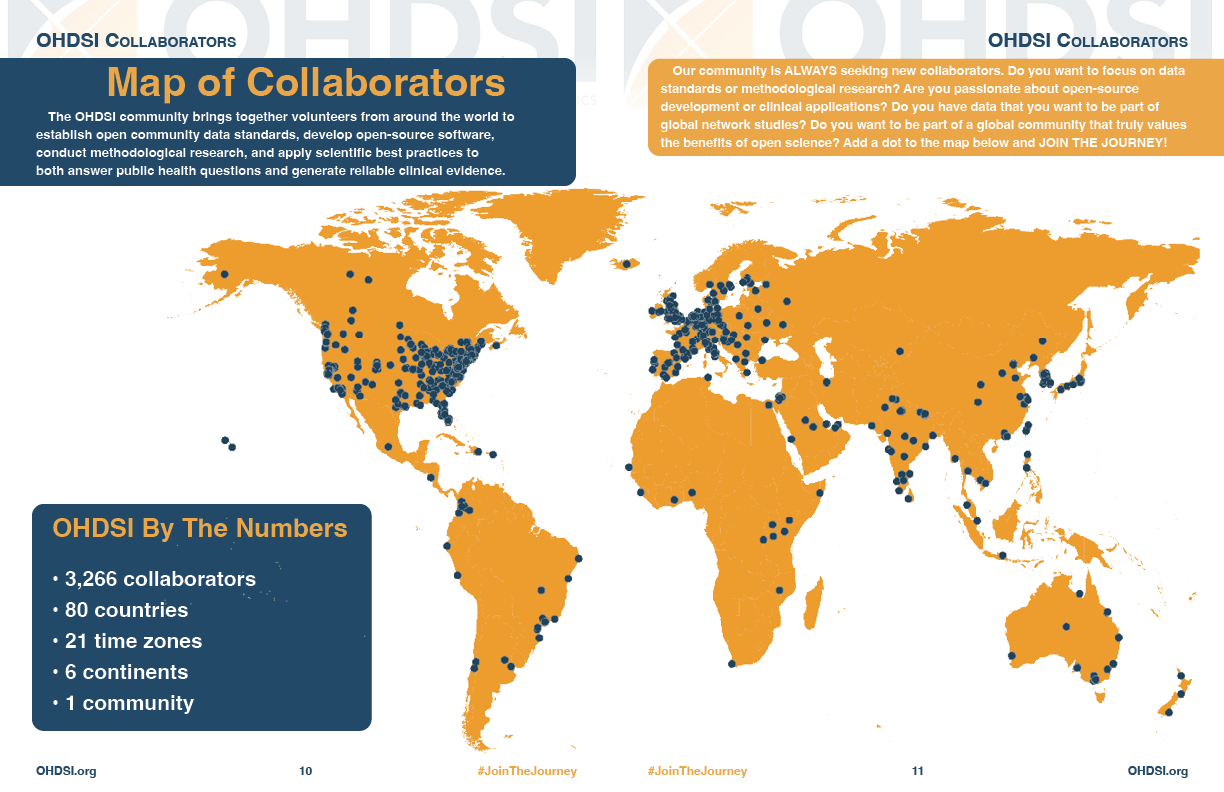
\includegraphics[width=0.90\textwidth]{figures/OHDSIcollaborators.png}
     \caption{Mapa de colaboradores de OHDSI. Extraído de la web oficial \cite{OHDSIwebsite}}
    \label{fig:OHDSIcollaborators}
\end{figure}

La colaboración con OHDSI se realiza a través de las diferentes fuentes de información que aporta la organización. 

Por su característica de ciencia abierta, la información sobre OHDSI está espacida por toda la red de internet mediante publicaciones científicas \cite{OHDSIpublications}, tutoriales para principiantes, grabaciones de las reuniones semanales de la comunidad o las conferencias anuales a través de su canal de youtube \cite{OHDSIyt}, canales de mensajería abierta como discord \cite{OHDSIdiscordInvitation} o MS Teams \cite{OHDSIofficeForm}, cientos de repositorios de github con información técnica de cada herramienta \cite{OHDSIgithub} y los foros de la comunidad para solventar dudas y preguntas \cite{OHDSIforums}, entre otros. No obstante, las fuentes de mayor rigor para acceder a la información sobre la organización son la web oficial \cite{OHDSIwebsite} y el Libro de OHDSI \cite{OHDSIbook}.

Todo el mundo está inivitdo a colaborar. Join the journey. 

- Collaborative network across XX countries, organizations...
- Github....
- Community calls...
-  Symposium

- Importancia europea Tal y como se presenta en \ref{sec:01EstadoArte}: proyectos europeos

\section{¿Cómo generar evidencia?}

- A journey from data to evidence (buscar en la documentación de ohdsi)

\subsection{Building blocks of OHDSI}

(buscar en la documentación de ohdsi)


\subsection{Estandarización de los datos}

- OMOP CDM

- OMOP VOCABULARY

\subsection{Investigación metodológica}
%%ADEMAS DE SER LOS TRES MÉTODOS QUE OFRECE OHDSI PARA REALZIAR INVESTIGACIONNES SON 3 CASOS DE USOS
-Caracterizacion
-Estimacion a nivel de poblacion
-Prediccion a nivel de paciente

\section{Herramientas}
\subsection{ATLAS}

- Extensa descripción de ATLAS (versión actual, anteriores, uso, aspecto...)

- Diferentes tipos de ATLAS (demo, Broadsea, AWS..)

ATLAS ADEMÁS IMPLEMENTA INTRÍNSICAMENTE  DOS HERRAMIENTAS

-ATHENA (herramienta de busqueda en el vocabulario del CDM) actualemnte está implementada dentro de ATLAS/Search

- ACHILLES (data quality dashboard) también esta implementada actualmente dentro de ATLAS/Data source


\subsection{Otras herramientas}

breve descripción de cada una:

-HADES (herramientas de análisis pero en librerias R)

-WHITE-RABBIT y RABBIT-IN-A-HAND (para preparar las ETL)

USAGI (también para la ETL)
...

\section{Conclusiones}